\documentclass[12pt]{article}

\usepackage[a4paper,margin=1in]{geometry}
\usepackage{graphicx}
\usepackage{amsmath}
\usepackage{booktabs}
\usepackage{listings}
\usepackage{xcolor}
\usepackage{hyperref}

\hypersetup{
colorlinks=true,
linkcolor=blue,
urlcolor=blue
}

\lstset{
language=C,
basicstyle=\ttfamily\small,
keywordstyle=\color{blue},
commentstyle=\color{green!60!black},
stringstyle=\color{red},
numbers=left,
numberstyle=\tiny,
stepnumber=1,
numbersep=5pt,
frame=single,
breaklines=true,
showstringspaces=false
}
\begin{document}

\begin{minipage}{0.6\textwidth}

\includegraphics[width=0.75\textwidth]{IIITB-COMET-Logo.png}
\end{minipage}
\begin{minipage}{0.38\textwidth}
\begin{center}
\textbf{DARSI VAMSI}
\newline
\textbf{COMET FWC 071}
\end{center}
\end{minipage}\\
\Large{\textbf{Implementation of Three LED Blinking using VAMAN ARM Development Board}}


\section{Objective}

The objective of this experiment is to verify the General Purpose Input Output (GPIO) functionality of the VAMAN ARM Development Board by blinking three LEDs sequentially. The experiment demonstrates GPIO initialization, digital output control, and software-based timing delays.

\section{Hardware Requirements}

\begin{enumerate}
\item VAMAN ARM Development Board
\item USB Cable
\item Three On-board LEDs
\item Ubuntu 24.04 LTS System
\item GNU ARM Embedded Toolchain
\end{enumerate}


\section{Software Requirements}

\begin{enumerate}
\item Ubuntu 24.04 LTS
\item GCC ARM Compiler
\item Make Utility
\item Serial Programming Tool
\item Makefile Build System
\end{enumerate}


\section{GPIO Configuration}

The following GPIO pins are configured as digital outputs.

\begin{table}[h]
\centering
\begin{tabular}{cc}
\toprule
GPIO Pin & Function\\
\midrule
GPIO 5 & LED 1\\
GPIO 10 & LED 2\\
GPIO 15 & LED 3\\
\bottomrule
\end{tabular}
\caption{GPIO Configuration}
\end{table}

\section{Program Description}

The application begins by configuring GPIO pins 5, 10, and 15 as output pins using the GPIO driver library.

Inside the infinite loop, each LED is turned ON one at a time while the remaining LEDs remain OFF. A software delay of 500 milliseconds is introduced after each LED transition, creating a continuous sequential blinking pattern.

The execution order is:

\begin{enumerate}
\item LED 1 ON
\item LED 2 ON
\item LED 3 ON
\item Repeat indefinitely
\end{enumerate}

\section{Algorithm}

\begin{enumerate}
\item Initialize the GPIO subsystem.
\item Configure GPIO 5 as Output.
\item Configure GPIO 10 as Output.
\item Configure GPIO 15 as Output.
\item Turn ON LED connected to GPIO 5.
\item Wait for 500 ms.
\item Turn ON LED connected to GPIO 10.
\item Wait for 500 ms.
\item Turn ON LED connected to GPIO 15.
\item Wait for 500 ms.
\item Repeat the sequence continuously.
\end{enumerate}


\section{Program}

\begin{lstlisting}
#include "gpio.h"
#include "delay.h"

void SystemInit(void)
{
}

int main(void)
{
    PyHal_GPIO_SetDir(5,1);
    PyHal_GPIO_SetDir(10,1);
    PyHal_GPIO_SetDir(15,1);

    while(1)
    {
        PyHal_GPIO_Set(5,1);
        PyHal_GPIO_Set(10,0);
        PyHal_GPIO_Set(15,0);
        delay_ms(500);

        PyHal_GPIO_Set(5,0);
        PyHal_GPIO_Set(10,1);
        PyHal_GPIO_Set(15,0);
        delay_ms(500);

        PyHal_GPIO_Set(5,0);
        PyHal_GPIO_Set(10,0);
        PyHal_GPIO_Set(15,1);
        delay_ms(500);
    }
}

void _start(void)
{
    main();

    while(1)
    {
    }
}
\end{lstlisting}

\section{Testing Procedure}

\begin{enumerate}
\item Connect the VAMAN ARM Development Board to the Ubuntu system.
\item Open the project directory.
\item Compile the project using the Makefile.
\item Generate the binary executable.
\item Flash the binary into the VAMAN ARM board.
\item Reset the board.
\item Observe the LEDs on the board.
\item Verify that the LEDs blink sequentially every 500 ms.
\end{enumerate}


\section{Expected Output}

The LEDs should blink in the following sequence.

\begin{center}
LED 1 $\rightarrow$ LED 2 $\rightarrow$ LED 3 $\rightarrow$ Repeat
\end{center}

Each LED remains ON for approximately 500 milliseconds before the next LED is activated.


\section{Observation}

\begin{itemize}
\item GPIO pins were successfully configured as outputs.
\item LEDs responded correctly to GPIO HIGH and LOW signals.
\item The software delay produced a visible blinking interval of approximately 500 ms.
\item Only one LED remained ON at any instant.
\end{itemize}


\section{Result}

The Three LED Blinking program was successfully implemented and executed on the VAMAN ARM Development Board. The GPIO driver correctly controlled the three LEDs, and the sequential blinking verified the proper functioning of the GPIO interface, software delay routine, and program execution flow.\\
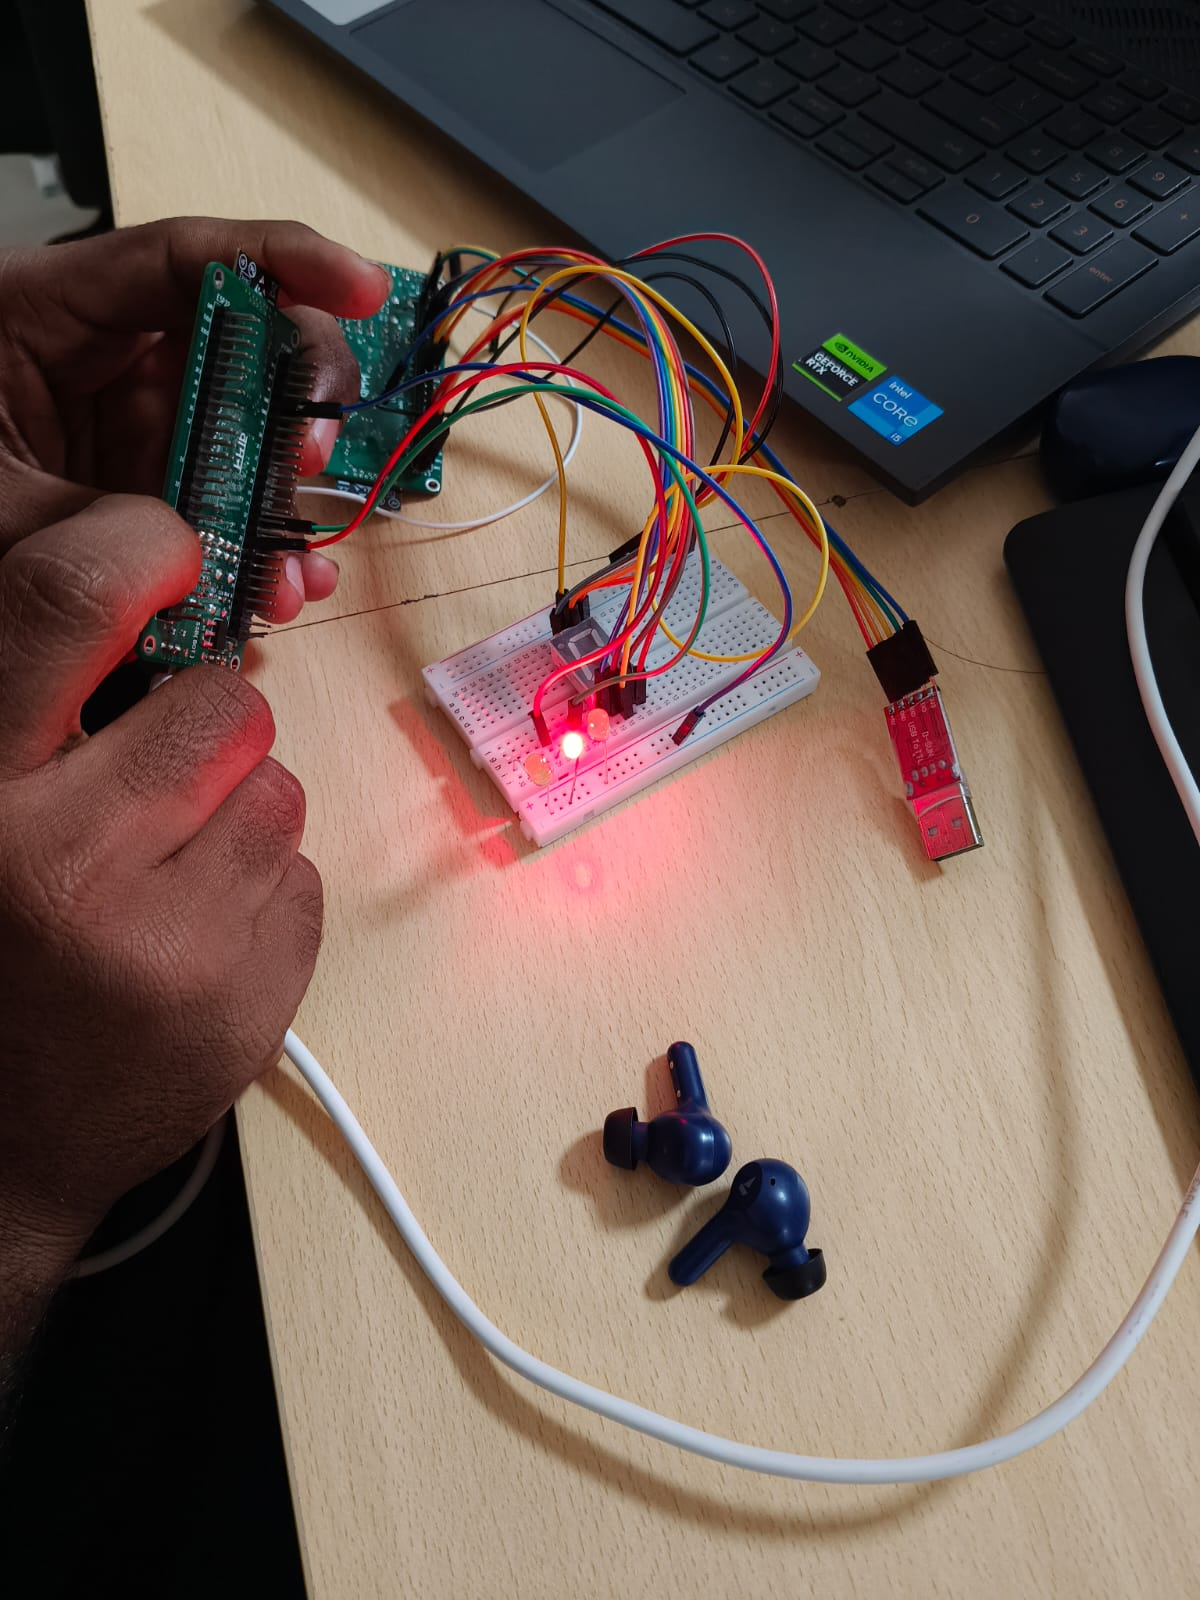
\includegraphics[width=0.55\textwidth]{three lked blink.jpeg}


\end{document}
